\chapter{Adattamenti}
\section{Adattamento con Stub Serie}
\subsection{Metodo 1}
Poniamoci nella situazione in cui vogliamo collegare il carico $Z_l$ sulla linea \textbf{senza} \textbf{perdite}, con \textbf{impedenza} \textbf{caratteristica} $Z_0$:
\begin{center}
    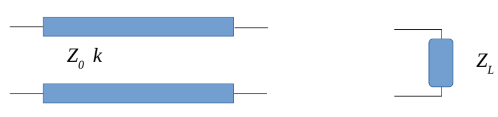
\includegraphics[width=0.8\textwidth]{Images/figure21.png}
\end{center}
Se la colleghiamo direttamente, avremo un \textbf{coefficiente di riflessione} non nullo:
\begin{equation*}
    \Gamma_l = \frac{Z_l - Z_0}{Z_l + Z_0}
\end{equation*}
E un \textbf{ROS} pari a:
\begin{equation*}
    ROS = \frac{1 + |\Gamma_l|}{1 - |\Gamma_l|}
\end{equation*}
Spostandosi lungo la linea, $|\Gamma|$ rimane \textbf{costante}, mentre il \textbf{modulo dell'impedenza} cambia sezione per sezione:
\begin{equation*}
    \frac{Z_0}{ROS} \leq |Z(z)| \leq Z_0 \ ROS
\end{equation*}
E analogamente la \textbf{parte reale dell'impedenza} varia tra:
\begin{equation*}
    \frac{Z_0}{ROS} \leq R(z) \leq Z_0 \ ROS   
\end{equation*}
In particolare esiste una coordinata $z'$ tale che:
\begin{equation*}
    R(z') = Z_0
\end{equation*}
E allo stesso tempo:
\begin{equation*}
    Z(z') = Z_0 + j \underbrace{X(z')}_{X_s}
\end{equation*}
\begin{center}
    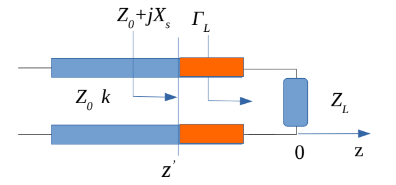
\includegraphics[width=0.7\textwidth]{Images/figure22.png}
\end{center}
\textbf{Ma come posso individuare questa sezione $z'$?\\ \\
}Ricordiamo che:
\begin{equation*}
\begin{aligned}
     Z(z') &= Z_0 \ \frac{1 + \Gamma(z')}{1 - \Gamma(z')} = Z_0 \ \frac{[1 + \Gamma(z')][1 - {\Gamma(z')}^*]}{{|1 - \Gamma(z')|}^2} =\\
     &= Z_0 \ \frac{1 - |\Gamma|^2 + 2j Im\{\Gamma(z')\}}{|1 - \Gamma(z')|^2} =\\
     &=Z_0 \ \frac{1 - |\Gamma|^2 }{|1 - \Gamma(z')|^2} + j Z_0 2 \frac{Im\{\Gamma(z')\}}{|1 - \Gamma(z')|^2}
\end{aligned}
\end{equation*}
Quindi affinchè:
\begin{equation*}
    R(z') = Z_0 \leftrightarrow \frac{1 - |\Gamma|^2 }{|1 - \Gamma(z')|^2} = 1
\end{equation*}
(se $|\Gamma|=1$ la linea è chiusa su una pura reattanza)\\ \\
Se $|\Gamma|<1$:
\begin{equation*}
    \begin{aligned}
    &1 - {|\Gamma|}^2 = {|1 - \Gamma(z')|}^2 = [1 - \Gamma(z')][1 - {\Gamma(z')}^*] = \\
    &= 1 - {\Gamma(z')}^* - \Gamma(z') + {|\Gamma|}^2 = 1 - 2Re\{\Gamma(z')\} + {|\Gamma|}^2
    \end{aligned}
\end{equation*}
Quindi:
\begin{equation*}
    Re\{\Gamma(z')\} = |\Gamma|^2 = |\Gamma_l|^2
\end{equation*}
Ricordando che:
\begin{equation*}
    \begin{aligned}
    \Gamma(z) &= \Gamma(0) e^{2jkz} = \Gamma_l e^{2jkz} = |\Gamma_l| e^{j\varphi_l} e^{2jkz} =|\Gamma_l| e^{j(2kz +\varphi_l)} =\\
    &= |\Gamma_l| \cos(2kz +\varphi_l) + j |\Gamma_l| \sin(2kz +\varphi_l)
    \end{aligned}
\end{equation*}
Quindi sostituendo otterremo:
\begin{equation*}
    Re\{\Gamma(z')\} = |\Gamma_l| \cos(2kz' +\varphi_l) = |\Gamma|^2 \implies \cos(2kz' +\varphi_l) = |\Gamma|
\end{equation*}
Che ha come soluzioni:
\begin{equation*}
    2k z'_n = \frac{4\pi}{\lambda} \pm ar\cos(|\Gamma_n|) - \varphi_l + 2n\pi
\end{equation*}
\begin{equation*}
    \implies z'_n = \pm \frac{ar\cos(|\Gamma_n|)}{2\pi} \frac{\lambda}{2} - \frac{\varphi_l}{2\pi} \frac{\lambda}{2} + n \frac{\lambda}{2} \ \forall n \ : \ z'_n <0
\end{equation*}
Quindi abbiamo trovato le ascisse $z'_n$ in corrispondenza delle quali:
\begin{equation*}
    Z(z'_n) = Z_0 + j Z_0 2 \frac{Im\{\Gamma(z'_n)\}}{|1 - \Gamma(z'_n)|^2}
\end{equation*}
Ricordando anche che:
\begin{itemize}
    \item $1 - |\Gamma_l|^2 = |1 - \Gamma(z_n')|^2 $
    \item $Im\{\Gamma(z'_n)\} = |\Gamma_l| \sin(2kz'_n +\varphi_l) = \pm \sqrt{1 - |\Gamma_l|^2}$
\end{itemize}

Quindi:
\begin{equation*}
    X_s = Im\{Z(z'_n)\} = Z_0 2 \frac{Im\{\Gamma(z'_n)\}}{|1 - \Gamma(z'_n)|^2} =  \pm Z_0 \underbrace{\frac{\sqrt{1 - |\Gamma_l|^2}}{1 - |\Gamma_l|^2}}_{\frac{\sqrt{X}}{X} = \frac{1}{\sqrt{X}}} = \frac{\pm Z_0}{\sqrt{1 - |\Gamma_l|^2}}
\end{equation*}
Quindi per ottenere l'adattamento dobbiamo \textbf{compensare} la $X_s$ inserendo a $z'_n$ una $X_s$ \textbf{uguale} ed \textbf{opposta}:
\begin{center}
    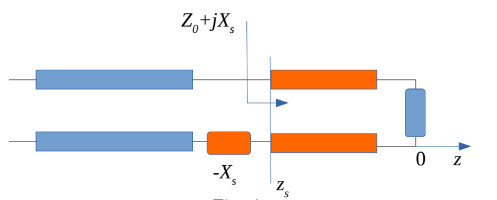
\includegraphics[width=0.7\textwidth]{Images/figure23.png}
\end{center}
La \textbf{reattanza} $X_s$ può essere realizzata con uno \textbf{stub in corto} o con \textbf{uno stub aperto} (es.\ corto):
\begin{center}
    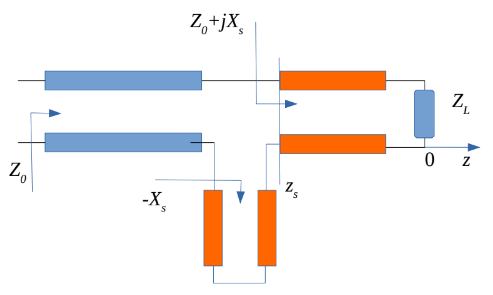
\includegraphics[width=0.7\textwidth]{Images/figure24.png}
\end{center}
\textbf{Ma a che distanza devo mettere lo stub??}\\ \\
\begin{equation*}
    Z(l) = j Z_0 \tan(kl)
\end{equation*}
Quindi pongo:\footnote{La tangente si annulla ogni $n\pi$}
\begin{equation*}
   Z_0 \tan(kl_{stub}) = - X_s
\end{equation*}
\begin{equation*}
  \implies l_{stub} = - atan\left(\frac{X_s}{Z_0}\right) \frac{\lambda}{2\pi} + n \frac{\lambda}{2} \geq 0
\end{equation*}
\subsection{Metodo 2}
Gli stessi risultati li possiamo ottenere con il \textbf{trasporto di impedenza}:\\ \\
Voglio trovare tutte le sezioni in cui \textbf{l'impedenza di carico trasportata ha parte reale $Z_0$}.
\begin{equation*}
    Z(l) = Z_0 \frac{R_l + j Z_0 \tan(kl)}{Z_0 + j R_l \tan(kl)} = Z_0 + j X_s
\end{equation*}
Divido primo e secondo membro per $Z_0$ e numeratore e denominatore per $Z_0$:
\begin{equation*}
    Z'(l) = \frac{R'_l + j t}{1 + j R'_l t} = 1 + j X'_s
\end{equation*}
Dove:
\begin{itemize}
    \item $Z'(l) = \frac{Z(l)}{Z_0}$
    \item $R'(l) = \frac{R_l}{Z_0}$
    \item $X'_s = \frac{X_s}{Z_0}$
    \item $t = \tan(kl)$
\end{itemize}
In particolare:
\begin{equation*}
    \begin{dcases}
    Re\{Z'(l)\} = 1\\
    Im\{Z'(l)\} = X'_s
    \end{dcases}
\end{equation*}
Cerchiamo ora di separare \textbf{parte} \textbf{reale} e \textbf{parte} \textbf{immaginaria}:
\begin{equation*}
    Z'(l) = \frac{(R'_l + j t)(1 - j R'_l t)}{1 +  {R'_l}^2 t^2} = \frac{R'_l - j {R'_l}^2 + jt + R'_l t^2 }{1 + {R'_l}^2 t^2} = 1 + j X'_s
\end{equation*}
Quindi:
\begin{equation*}
    \frac{R'_l + R'_l t^2}{1 +  {R'_l}^2 t^2} = 1
\end{equation*}
\begin{equation*}
    \frac{- {R'_l}^2 t +t}{1 + {R'_l}^2 t^2} = X'_s
\end{equation*}
\textbf{Risolviamo la prima in t}:\\ 
Ricordiamoci però che la vera incognita è l!!\\ \\
Quindi per prima cosa verifichiamo se $t=\infty$, ovvero $l = \frac{\lambda}{4}$ è \textbf{soluzione del problema}:
\begin{equation*}
    t=\infty \implies Z\left(\frac{\lambda}{4}\right) \approx \frac{1}{R'_l} = 1
\end{equation*}
Ma questo può accadere solo se $R'_l = 1$, quindi\textbf{ NON è soluzione.}\\ \\
Procediamo quindi moltiplicando per $1 + {R'_l}^2 t^2$:
\begin{equation*}
    R'_l + {R'_l} t^2= 1 + {R'_l}^2 t^2 \implies ( {R'_l}^2 - R'_l) t^2 = R'_l -1
\end{equation*}
\begin{equation*}
    \implies t^2 = \frac{R'_l -1}{{R'_l}^2 - R'_l} \implies t^2 = \frac{\cancel{R'_l -1}}{R'_l\cancel{({R'_l} - 1)}} = \frac{1}{R'_l} \implies t = \frac{1}{\sqrt{R'_l}}
\end{equation*}
\begin{equation*}
    \implies \tan(kl) = t = \pm \sqrt{\frac{1}{{R'_l}}} = \pm \sqrt{\frac{Z_0}{R_l}}
\end{equation*}
Da questa espressione valuto la l in corrispondenza della quale:
\begin{equation*}
    Z(l) = Z_0 + j X_s
\end{equation*}
Ovvero:
\begin{equation*}
    l = \\arctan\left(\sqrt{\frac{Z_0}{R_l}}\right) \frac{\lambda}{2\pi} + n \frac{\lambda}{2} \geq 0
\end{equation*}
Una volta calcolata la l alla quale vogliamo fare l'adattamento mi ricavo $X_s$:
\begin{equation*}
    \begin{aligned}
    X'_s &= \frac{- {R'_l}^2 t +t}{1 + {R'_l}^2 t^2} = \frac{\pm (1 - {R'_l}^2) \sqrt{\frac{1}{R'_l}}}{1 + R'_l} = \pm \frac{\frac{1 - {R'_l}^2}{\sqrt{R'_l}}}{1 + R'_l} =\\
    &= \pm \frac{1 -{R'_l}^2 }{\sqrt{R'_l} (1 +{R'_l})} = \pm \frac{(1 -{R'_l})\cancel{(1 +{R'_l})}}{\sqrt{R'_l} \cancel{(1 +{R'_l})}} = \pm \frac{1 - {R'_l}}{\sqrt{R'_l}}
    \end{aligned}
\end{equation*}
Quindi:
\begin{equation*}
    X_s = X'_s \cdot \underbrace{Z_0}_{R_0} = \pm \frac{1 - \frac{R_l}{Z_0}}{\sqrt{\frac{R_l}{Z_0}}} \cdot Z_0 = \pm \frac{Z_0 - R_l}{\sqrt{R_l} / \sqrt{Z_0}} = \pm (R_0 - R_l) \cdot \sqrt{\frac{R_0}{R_l}}
\end{equation*}
Questa \textbf{reattanza} va compensata con una \textbf{reattanza} \textbf{uguale} e \textbf{opposta} attraverso uno \textbf{stub serie}:
\begin{equation*}
    X_{stub} = Z_0 \tan(kl_{stub}) = - X_s
\end{equation*}
\begin{equation*}
    kl_{stub} = -\arctan\left(\frac{X_s}{Z_0}\right) + n\pi
\end{equation*}
\begin{equation*}
   \implies l_{stub} = -\arctan\left(\frac{X_s}{Z_0}\right) \frac{\lambda}{2\pi} + n \frac{\lambda}{2} \geq 0
\end{equation*}

\section{Adattamento con Stub Parallelo}
\subsection{Metodo 1}
Nel caso di un \textbf{adattamento} mediante \textbf{stub parallelo} conviene lavorare con le \textbf{ammettenze}.\\
Consideriamo quindi una linea \textbf{senza perdite} con un'\textbf{ammettenza caratteristica} $Y_0 = \frac{1}{Z_0}$ che vogliamo collegare ad un carico di \textbf{ammettenza} $Y_l = \frac{1}{Z_l}$:
\begin{center}
    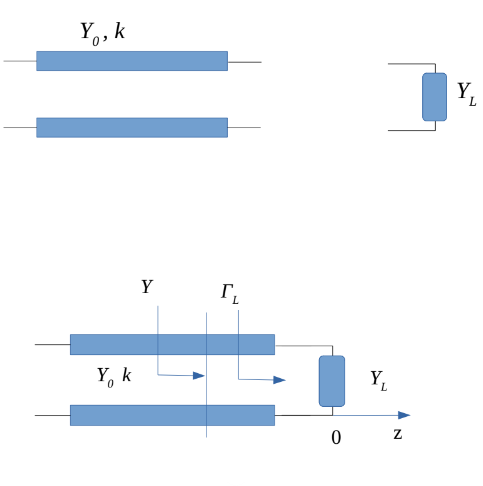
\includegraphics[width=0.7\textwidth]{Images/figure25.png}
\end{center}
Ricordiamo che:
\begin{equation*}
\begin{aligned}
     Y(z') &= Y_0 \ \frac{1 - \Gamma(z')}{1 + \Gamma(z')} = Y_0 \ \frac{[1 - \Gamma(z')][1 + {\Gamma(z')}^*]}{{|1 + \Gamma(z')|}^2} =\\
     &= Y_0 \ \frac{1 - |\Gamma|^2 - 2j Im\{\Gamma(z')\}}{|1 + \Gamma(z')|^2} =\\
     &=Y_0 \ \frac{1 - |\Gamma|^2 }{|1 + \Gamma(z')|^2} - j Y_0 2 \frac{Im\{\Gamma(z')\}}{{|1 + \Gamma(z')|}^2}
\end{aligned}
\end{equation*}
Quindi affinchè:
\begin{equation*}
    Y(z') = G(z') + j B(z') = Y_0 + j B_p \leftrightarrow Y_0 \frac{1 - |\Gamma|^2 }{|1 + \Gamma(z')|^2} = Y_0
\end{equation*}
(se $|\Gamma|=1$ la linea è chiusa su una pura reattanza)
Se $|\Gamma|<1$:
\begin{equation*}
    \begin{aligned}
    &1 - {|\Gamma|}^2 = {|1 + \Gamma(z')|}^2 = [1 + \Gamma(z')][1 + {\Gamma(z')}^*] = \\
    &= 1+ {\Gamma(z')}^* + \Gamma(z') + |\Gamma|^2 = 1 + 2Re\{\Gamma(z')\} + |\Gamma|^2
    \end{aligned}
\end{equation*}
Quindi:
\begin{equation*}
    Re\{\Gamma(z')\} = -|\Gamma|^2 = -|\Gamma_l|^2
\end{equation*}
Ricordando che:
\begin{equation*}
    \begin{aligned}
    \Gamma(z) &= \Gamma(0) e^{2jkz} = \Gamma_l e^{2jkz} = |\Gamma_l| e^{j\varphi_l} e^{2jkz} =|\Gamma_l| e^{j(2kz +\varphi_l)} =\\
    &= |\Gamma_l| \cos(2kz +\varphi_l) + j |\Gamma_l| \sin(2kz +\varphi_l)
    \end{aligned}
\end{equation*}
Quindi sostituendo otterremo:
\begin{equation*}
    Re\{\Gamma(z')\} = |\Gamma_l| \cos(2kz' +\varphi_l) = -|\Gamma|^2 \implies \cos(2kz' +\varphi_l) = -|\Gamma|
\end{equation*}
Che ha come \textbf{soluzioni}:
\begin{equation*}
    2k z'_n = \frac{4\pi}{\lambda} \pm ar\cos(-|\Gamma_n|) - \varphi_l + 2n\pi
\end{equation*}
\begin{equation*}
    \implies z'_n = \pm \frac{ar\cos(-|\Gamma_n|)}{2\pi} \frac{\lambda}{2} - \frac{\varphi_l}{2\pi} \frac{\lambda}{2} + n \frac{\lambda}{2} \ \forall n \ : \ z'_n <0
\end{equation*}
Che sono le \textbf{ascisse} in cui $G = Y_0$.\\ \\
Ripetendo calcoli analoghi:
\begin{equation*}
    Im\{\Gamma(z'_n)\} = |\Gamma_l| \sin(2kz'_n +\varphi_l) = \pm \sqrt{1 - |\Gamma_l|^2}
\end{equation*}
Quindi:
\begin{equation*}
    B_p = Im\{Y(z'_n)\} = Y_0 2 \frac{Im\{\Gamma(z'_n)\}}{|1 + \Gamma(z'_n)|^2} = \pm Y_0 \frac{\sqrt{1 - |\Gamma_l|^2}}{1 - |\Gamma_l|^2} = \frac{\pm Y_0}{\sqrt{1 - |\Gamma_l|^2}}
\end{equation*}
Quindi ora per ottenere l'\textbf{adattamento} devo compensare la \textbf{suscettanza} $B_p$ con una \textbf{suscettanza} \textbf{uguale} ed \textbf{opposta}, attraverso per esempio uno \textbf{stub parallelo} in corto:
\begin{center}
    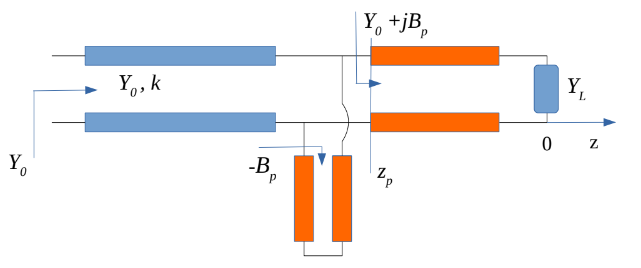
\includegraphics[width=0.7\textwidth]{Images/figure26.png}
\end{center}
\subsection{Metodo 2}
Gli stessi risultati li possiamo ottenere con il \textbf{trasporto di ammettenza}:\\ \\
Voglio trovare tutte le sezioni in cui l'\textbf{ammettenza} di carico \textbf{trasportata} ha \textbf{parte reale} $G_L$.
\begin{equation*}
    Y(l) = Y_0 \frac{Y_l + j Y_0 \tan(kl)}{Y_0 + j Y_l \tan(kl)} = Y_0 + j B_p
\end{equation*}
Divido primo e secondo membro per $Y_0$ e numeratore e denominatore per $Y_0$:
\begin{equation*}
    Y'(l) = \frac{G'_l + j t}{1 + j G'_l t} = 1 + j B_p
\end{equation*}
Dove:
\begin{itemize}
    \item $Y'(l) = \frac{Y(l)}{Y_0}$
    \item $G'_l = \frac{G_l}{Y_0}$
    \item $B'_p = \frac{B_p}{Y_0}$
    \item $t = \tan(kl)$
\end{itemize}
In particolare:
\begin{equation*}
    \begin{dcases}
    Re\{Y'(l)\} = 1\\
    Im\{Y'(l)\} = B'_P
    \end{dcases}
\end{equation*}
Cerchiamo ora di separare \textbf{parte} \textbf{reale} e \textbf{parte} \textbf{immaginaria}:
\begin{equation*}
    Y'(l) = \frac{(G'_l + j t)(1 - j G'_l t)}{1 + j {G'_l}^2 t^2} = \frac{G'_l - j {G'_l}^2 + jt + G'_l t^2 }{1 + j {G'_l}^2 t^2} = 1 + j B'_P
\end{equation*}
Quindi:
\begin{equation*}
    \frac{G'_l + G'_l t^2}{1 + j {G'_l}^2 t^2} = 1
\end{equation*}
\begin{equation*}
    \frac{- {G'_l}^2 t +t}{1 + {G'_l}^2 t^2}
\end{equation*}
Risolviamo la prima in t:\\ 
Procediamo quindi moltiplicando per $1 + {G'_l}^2 t^2$:
\begin{equation*}
    G'_l + {G'_l}^2 = 1 + {G'_l}^2 t^2 \implies ( {G'_l}^2 - G'_l) t^2 = G'_l -1
\end{equation*}
\begin{equation*}
    \implies t^2 = \frac{G'_l -1}{{G'_l}^2 - G'_l} \implies t^2 = \frac{G'_l -1}{G'_l\cancel{({G'_l} - 1)}} = \frac{1}{G'_l} \implies t = \frac{1}{\sqrt{G'_l}}
\end{equation*}
\begin{equation*}
    \implies \tan(kl) = t = \pm \sqrt{\frac{1}{{G'_l}}} = \pm \sqrt{\frac{Y_0}{G_l}}
\end{equation*}
Da questa espressione valuto la l in corrispondenza della quale:
\begin{equation*}
    Y(l) = Y_0 + j B_p
\end{equation*}
Ovvero:
\begin{equation*}
    l = \arctan\left(\frac{Y_0}{G_l}\right) \frac{\lambda}{2\pi} + n \frac{\lambda}{2} \geq 0
\end{equation*}
Una volta calcolata la l alla quale vogliamo fare l'\textbf{adattamento} mi ricavo $B_p$:
\begin{equation*}
    \begin{aligned}
    B'_p &= \frac{- {G'_l}^2 t +t}{1 + {G'_l}^2 t^2} = \frac{\pm (1 - {G'_l}^2) \sqrt{\frac{1}{G'_l}}}{1 + G'_l} = \pm \frac{\frac{1 - {G'_l}^2}{\sqrt{G'_l}}}{1 + G'_l} =\\
    &= \pm \frac{1 -{G'_l}^2 }{\sqrt{G'_l} (1 +{G'_l})} = \pm \frac{(1 -{G'_l})\cancel{(1 +{G'_l})}}{\sqrt{G'_l} \cancel{(1 +{G'_l})}} = \pm \frac{1 - {G'_l}}{\sqrt{G'_l}}
    \end{aligned}
\end{equation*}
Quindi:
\begin{equation*}
    B_p = B'_p \cdot Y_0 = \pm \frac{1 - \frac{G_l}{Y_0}}{\sqrt{\frac{G_l}{Y_0}}} \cdot Y_0 = \pm \frac{Y_0 - G_l}{\sqrt{G_l} / \sqrt{Y_0}} = \pm (Y_0 - G_l) \cdot \sqrt{\frac{Y_0}{G_l}}
\end{equation*}
Questa \textbf{reattanza} va \textbf{compensata} con una \textbf{reattanza} \textbf{uguale} e \textbf{opposta} attraverso uno \textbf{stub} \textbf{parallelo}:
\begin{equation*}
    B_{stub} = Y_0 co\tan(kl_{stub}) = - B_p
\end{equation*}
\begin{equation*}
    kl_{stub} = -arcotan\left(\frac{B_p}{Y_0}\right) + n\pi
\end{equation*}
\begin{equation*}
   \implies l_{stub} = -arcotan\left(\frac{B_p}{Y_0}\right) \frac{\lambda}{2\pi} + n \frac{\lambda}{2} \geq 0
\end{equation*}


\section{Adattamento Tramite Inverter}
Consideriamo la seguente \textbf{linea senza perdite chiusa su un carico}:
\begin{center}
    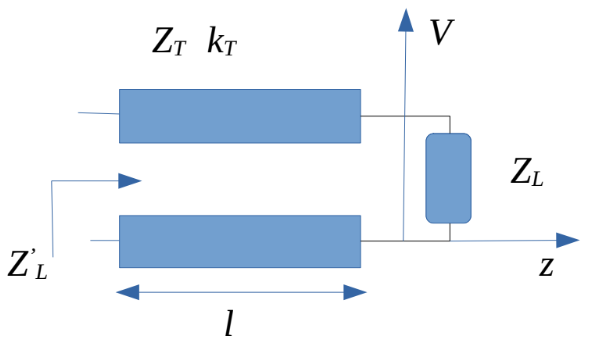
\includegraphics[width=.6\textwidth]{Images/figure43.png}
\end{center}
L'impedenza $Z'_L$ sarà:
\begin{equation*}
    Z'_L = Z_T \frac{Z_L + j Z_T \tan(k_T l)}{Z_T + j Z_L \tan(k_T l)}
\end{equation*}

Nel caso in cui:
\begin{equation*}
    k_T l = \frac{\pi}{2} \implies l = \frac{\lambda_T}{4}
\end{equation*}
Allora:
\begin{equation*}
    k_T l = \left(\frac{\pi}{2}\right) \longrightarrow \infty
\end{equation*}
Quindi va calcolata con il limite:
\begin{equation*}
    Z'_L = \lim\limits_{\tan(k_T l) \longrightarrow \infty} Z_T \frac{Z_L + j Z_T \tan(k_T l)}{Z_T + j Z_L \tan(k_T l)} = \frac{Z_T^2}{Z_L} = Z_T^2 Y_L
\end{equation*}
\textbf{Quindi possiamo dire che il trasporto di un'impedenza di un quarto di lunghezza d'onda lungo una linea da luogo ad un'impedenza proporzionale al reciproco dell'impedenza originale.}



